%****************************************************
%	CHAPTER 3 - THEORETICAL DEVELOPMENT
%****************************************************
\chapter{Theoretical Development}
\label{ch:theory}

%====================================================
\section{Optical Properties of Ice and Snow}
\label{sec:ch3:section1}

Ice and snow have more interactions with light than mediums typically observed by optical sensors, especially LIDAR which is typically used in urban environments or for terrain mapping. Not only is light reflected by ice and snow, but it can also pass through the mediums, as well as being refracted and absorbed.

%====================================================
\section{Robot Operating System (ROS)}
\label{sec:ch3:section2}

Robot Operating System (ROS), is a collection of open-source software tools that allows for the development of modular autonomous platforms. ROS is widely used in many environments, ranging from research and prototyping platforms to massive corporations such as Airbus and Caterpillar (cite here).
ROS allows hardware to be easily added and removed from a platform for testing and development. The Livox Avia has manufacturer-supplied ROS drivers, hence this was the chosen method for interfacing with the device during data collection. 

%====================================================
\section{Livox Avia}
\label{sec:ch3:section3}

The sensor used to collect data for this investigation was the Livox Avia. The Livox Avia is a solid-state laser and Risley prism-based LIDAR scanner with a built-in inertial measurement unit (IMU). ***this might have to move* The sensor was set up to capture data using ROS (ROS Neotic) and the Livox ROS driver through a machine running Ubuntu 20.04. The sensor scans and creates point clouds at a rate of 10 Hz and the IMU collects data at a rate of 200 Hz. The captured data was saved and stored in the rosbag file format (.bag). These files contain all the recorded data, (point cloud e here).information (location and return intensity), IMU readings, and their associated timestamps.***

%----------------------------------------------------
\begin{figure}[H]
    \centering
    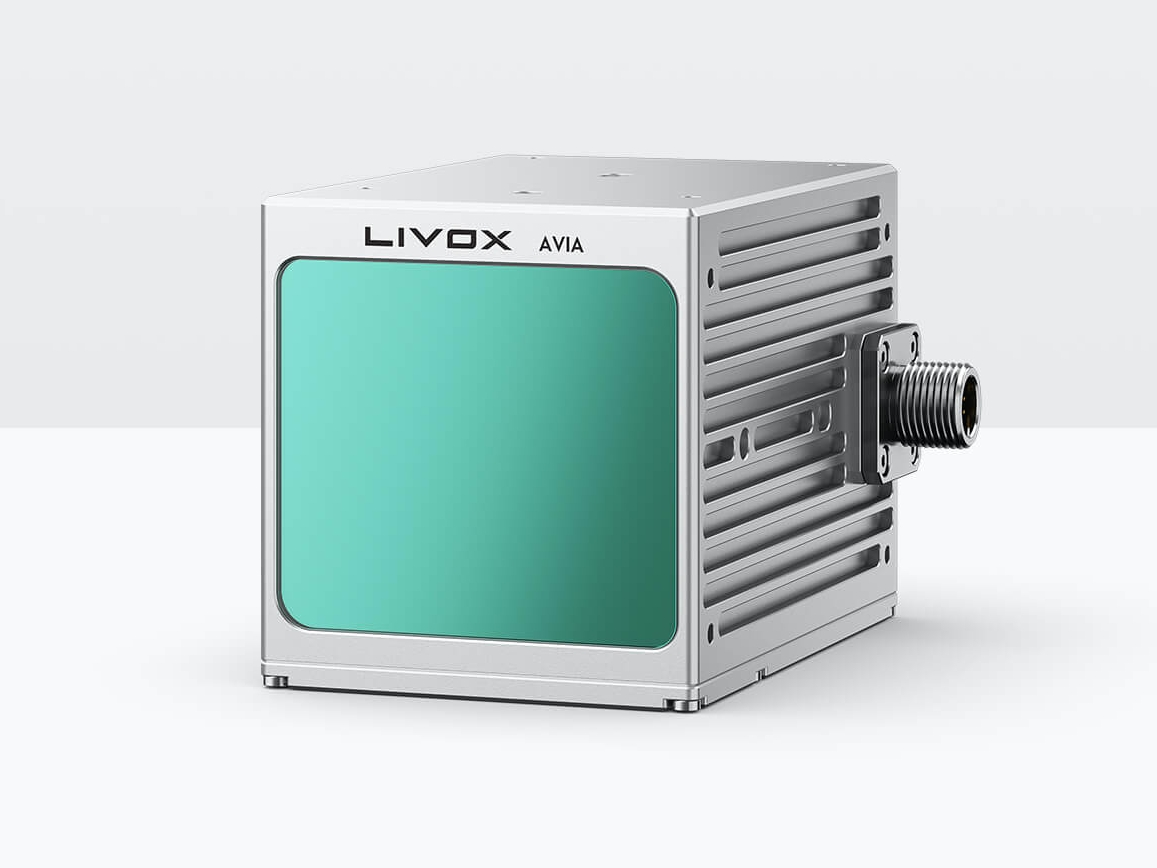
\includegraphics[width=0.5\textwidth]{figs/avia0.jpg}
    \caption{\textbf{Livox Avia}}
    \label{fig:avia}
\end{figure}
%----------------------------------------------------

The Avia has two built-in scanning patterns, a repetitive and a non-repetitive pattern. The repetitive scanning pattern scans the target area in a narrow horizontal band, providing a more uniform point density per frame when compared to the non-repetitive mode. The non-repetitive scanning pattern scans the target with a rosette-shaped pattern which rotates as it scans, covering areas not scanned in previous frames. This scanning method results in a high density of points in the centre of the target, with the number of points reducing towards the edges of the sensor's field of view (FOV). The non-repetitive scanning pattern was used for data capture as it provides a wider FOV than the non-repetitive scanning pattern and captures more unique data points.

\begin{figure}[H]
    \centering
    \begin{minipage}{0.33\textwidth}
        \centering
        
\includegraphics[width=1\textwidth]{figs/rep0.jpg} % first figure itself
        %\caption{first figure}
    \end{minipage}\hfill
    \begin{minipage}{0.33\textwidth}
        \centering
        
\includegraphics[width=1\textwidth]{figs/rep1.jpg} % second figure itself
        %\caption{second figure}
    \end{minipage}
    \begin{minipage}{0.33\textwidth}
        \centering
        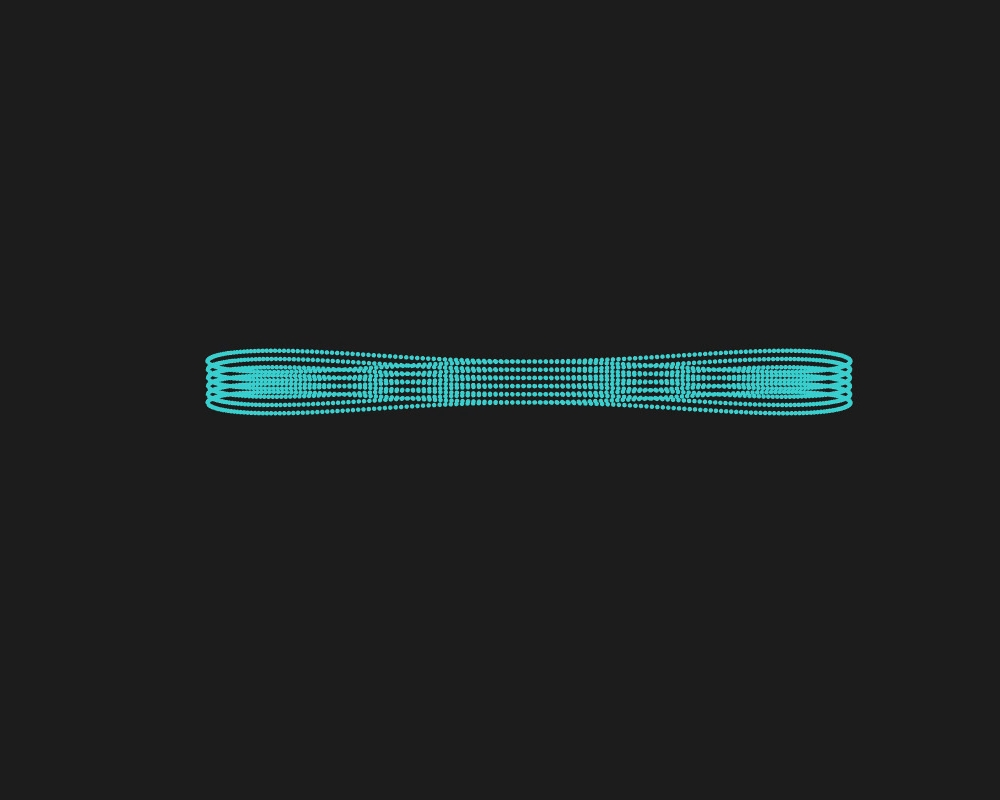
\includegraphics[width=1\textwidth]{figs/rep2.jpg} % first figure itself
        %\caption{first figure}
    \end{minipage}\hfill
    \caption{\textbf{Livox Avia Repetitive Scanning Pattern}}
    \label{fig:rep}
\end{figure}

\begin{figure}[H]
    \centering
    \begin{minipage}{0.33\textwidth}
        \centering
        
\includegraphics[width=1\textwidth]{figs/norep0.jpg} % first figure itself
        %\caption{first figure}
    \end{minipage}\hfill
    \begin{minipage}{0.33\textwidth}
        \centering
        
\includegraphics[width=1\textwidth]{figs/norep1.jpg} % second figure itself
        %\caption{second figure}
    \end{minipage}
    \begin{minipage}{0.33\textwidth}
        \centering
        
\includegraphics[width=1\textwidth]{figs/norep2.jpg} % first figure itself
        %\caption{first figure}
    \end{minipage}\hfill
    \caption{\textbf{Livox Avia Non-Repetitive Scanning Pattern}}
    \label{fig:non_rep}
\end{figure}


The sensor has three return rate settings: single, double, or triple return. The Avia was used exclusively in single return mode.

\begin{table}[H]
\centering
\begin{tabular}{lllll}
\cline{1-2}
Laser Wavelength            & 905 nm                                     &  &  &  \\ \cline{1-2}
Laser Safety                & Class 1 (Safe for eyes)                    &  &  &  \\ \cline{1-2}
Detection Range (@ 100 klx) & \begin{tabular}[c]{@{}l@{}}190 m @ 10\% reflectivity\\ 230 m @ 20\% reflectivity\\ 320 m @ 80\% reflectivity\end{tabular} &  &  &  \\ \cline{1-2}
Detection Range (@ 0 klx)   & \begin{tabular}[c]{@{}l@{}}190 m @ 10\% reflectivity\\ 260 m @ 20\% reflectivity\\ 450 m @ 80\% reflectivity\end{tabular} &  &  &  \\ \cline{1-2}
FOV                         & \begin{tabular}[c]{@{}l@{}} Non-repetitive Scanning Pattern: 70.4° (H) × 77.2 (V)\\ Repetitive Scanning Pattern: 70.4° (H) × 4.5° (V)\end{tabular}          &  &  &  \\ \cline{1-2}
Distance Random Error       & 1$\sigma$ (@ 20 m) $<$ 2 cm                         &  &  &  \\ \cline{1-2}
Point Rate                  & 240,000 points/s                           &  &  &  \\ \cline{1-2}
IMU                         & Bosch Sensortec BMI088                     &  &  &  \\ \cline{1-2}
Operating Temperature Range & -20° to 65° C                              &  &  &  \\ \cline{1-2}
IP Rating                   & IP67                                       &  &  &  \\ \cline{1-2}
Dimensions                  & 91 x 61.2 x 64.8 mm                        &  &  &  \\ \cline{1-2}
\end{tabular}
\caption{\textbf{Livox Avia Specifications.} The parameters}
\label{table:AVIA_spec}
\end{table}

%====================================================
\section{LIDAR Characteristics}
\label{sec:ch3:section4}

LIDAR is used over other remote sensing methods for various reasons. Being an active method is advantageous over visual method such as telephoto or stereoscopic cameras as it does not require external illumination to observe the target. Additionally, with the correct sensor selection, LIDAR is less susceptible to issues such as lens flare or overexposure to which typical cameras are prone. Certain LIDAR sensors also have the ability to penetrate vegetation, allowing mapping of ground surfaces beneath areas obscured by plant cover.\\
Compared to radar, LIDAR typically has superior mapping precision and target resolution, allowing more accurate reproductions of the target and the surrounding environment.
Using LIDAR is not without its disadvantages. LIDAR sensors are more expensive than more traditional remote sensing hardware. Unlike cameras, which can recover details such as colour, LIDAR is only able to recover the three-dimensional geometry of the target. Radar outperforms LIDAR in certain applications. It is capable of much larger detection ranges than LIDAR and is also unaffected by adverse environmental conditions such as smoke, rain, and fog.

BACKSCATTER?
REFLECTIVITY?
ABSORPTION?
Wavelength

%====================================================
\section{Point Cloud Processing}
\label{sec:ch3:section5}

Many common point cloud processing methods are built around the assumption that the point cloud being worked upon is in the format of a standard (M x N) grid layout. Methods such as point cloud registration (obtaining the transformation between two point clouds \cite{huangComprehensiveSurveyPoint2021}), clustering and model fitting often use the assumption of a constant grid with a constant number of points per frame to achieve their outputs. To bypass this limitation it is common for point clouds to be downsampled through a grid filter to achieve the desired format \cite{3DPointCloud}.

In the Avia's repetitive scanning pattern (See Figure \ref{fig:rep}), the sensor produces a point cloud with a roughly rectangular FOV and consistent point density, which is suitable for downsampling and grid filtering. Point clouds produced by the non-repetitive scanning pattern (See Figure \ref{fig:non_rep}) are circular and do not have uniform point density and are thus not ideal for downsampling and grid filtering.

Many processing methods are also based on the assumption that the environment data is collected from will contain predominantly objects made of simple geometries. For example, a scene in an urban environment will contain many objects made of rectangles, circles and triangles. The environment that data for this investigation was captured contains none of these simple shapes, with the geometry of the pancake floes being irregular and superimposed upon complex ocean surface waves.

%====================================================
\section{Kalman Filters}
\label{sec:ch3:section6}
The Kalman Filter is a recursive predictor-corrector algorithm used to provide optimal estimates of unknown variables of a system given various noisy measurements as inputs to the algorithm over time \cite{govaersIntroductionImplementationsKalman2019}. The method is named after Rudolph E. Kálmán, the engineer and mathematician who first described it in his now famous paper, \cite{kalmanNewApproachLinear1960}.

The Kalman filter uses the state-space format of a linear dynamic system, with the assumption that the measurements and process are subject to Gaussian noise.

The process model of the system over time $k-1$ to $k$ is given as:

%----------------------------------------------------
\begin{equation} \label{process}
    x_k = Fx_{k-1} + Bu_{k-1} + w_{k-1} \quad
\end{equation}
%----------------------------------------------------

where $F$ is the state transition matrix applied the previous state matrix ($x_{k-1}$), $B$ is the control-input matrix applied to the control input vector ($u_{k-1}$) and the vector $w_{k-1}$ represents the process noise, assumed to be zero-mean Gaussian with covariance of $Q$ such that $w_{k-1} \sim N(0, Q)$.

The measurement model describes the relation between the state and measurement of the system at time $k$ and is given as:

%----------------------------------------------------
\begin{equation} \label{measure}
    z_k = Hx_k + \nu_k \quad
\end{equation}
%----------------------------------------------------

where $H$ relates the current state ($x_{k}$)  to the measurement ($z_{k}$) and the vector $v_{k}$ represents the measurement noise, assumed to be zero-mean Gaussian with covariance of $R$ such that $v_{k} \sim N(0, R)$.

The filter consists of three states:

\begin{enumerate}
    \item Initialization
    \item Prediction
    \item Update
\end{enumerate}

Before beginning the main prediction loop, the filter first needs a guess of the initial state of the system:

%----------------------------------------------------
\begin{equation} \label{init_state}
    \hat{x}_0^+ \quad
\end{equation}



%====================================================
\section{Plane Fitting}
\label{sec:ch3:section7}


%====================================================
\section{Clustering Algorithms}
\label{sec:ch3:section8}

As a human, organising and sorting large amounts of objects or data into groups is often a trivial task that requires minimal mental exertion but significant time to complete. Automating this process can greatly reduce the time required to process a dataset, if implemented well. Selecting an algorithm or method will determine the accuracy, time and computing costs of automating the clustering process. Different methods are suited for use depending on properties of the data to be clustered (properties such as data dimensions, number of data points and the relationship between individual data points), knowledge of the final classes the data will be clustered into and computational restraints \cite{xuComprehensiveSurveyClustering2015}.

Clustering Algorithms can be categorised based on the methods by which they function, some of the most common categories are Partitional, Hierarchical, Density, Model-based and Spectral-based.
\\Partitional methods
\\Hierarchical methods are built upon the assumption that there is a hierarchical relationship between the data and the algorithm constructs this hierarchy, thus clustering the data.
\\Density based algorithms group areas of data with high density as individual clusters.
\\Model-based algorithms find the best fit of a pre-selected model to the data.